\subsection{Model Scaling Study}
\label{subsec:scalability}

\begin{figure}[t]
    \centering
    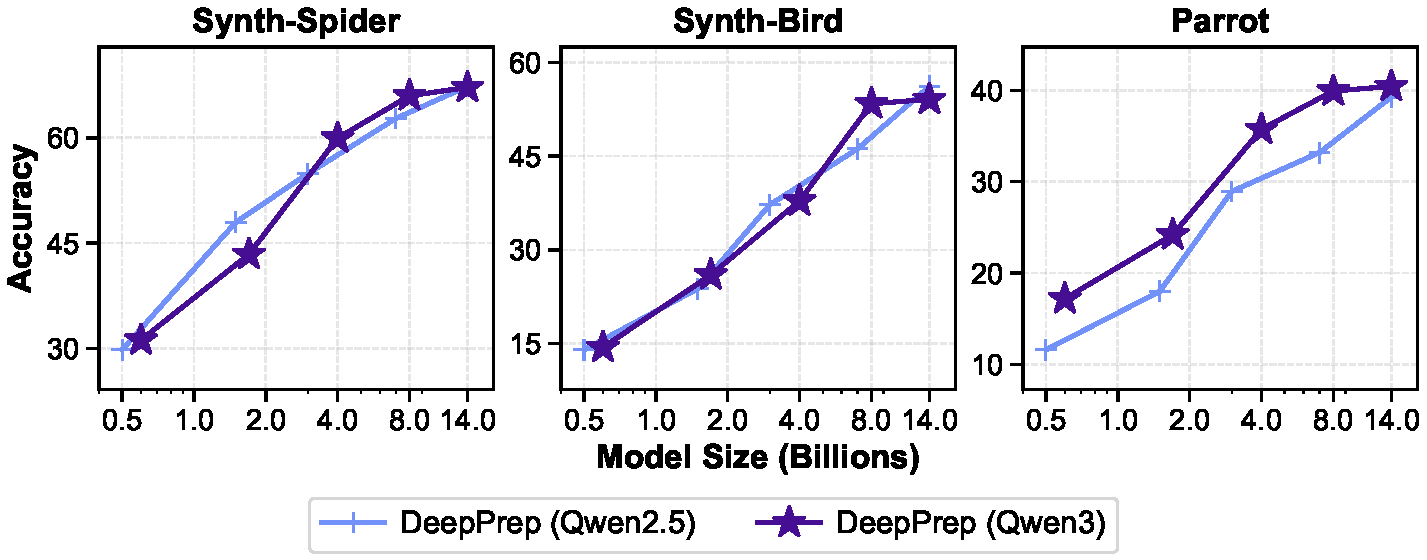
\includegraphics[width=1.01\columnwidth]{plots/plot/performance_scale_accuracy_only.pdf}
    \vspace{-1.5em} 
    \caption{Performance scales with larger model size.
    % \fmh{Results of Qwen2.5 are not updated (Use 2025 version).} 
    }
    \label{\labelprefix fig:performance_scale_accuracy_only}
    \vspace{-0.5em} 
  %\vspace{-1em}
\end{figure}

\stitle{Exp-\expnum\label{exp:model_scaling}: Model Scaling Study.}
We study how \sys performs under different backbone model sizes. We train \sys with LLM backbones ranging from 0.5B to 14B parameters across the Qwen2.5 and Qwen3 families.
Figure~\ref{\labelprefix fig:performance_scale_accuracy_only} shows that accuracy steadily increases with model size. On Synth-Spider, scaling Qwen3 from 0.6B to 14B improves Accuracy from 31.20 to 67.18. Across comparable model sizes, the Qwen3 series also shows stronger out-of-domain performance than Qwen2.5. For example, on Synth-Bird, Qwen3-8B achieves 53.39 Accuracy versus 46.17 for Qwen2.5-7B. These results suggest \sys benefits from stronger backbone models and maintains positive scaling trends.

%\noindent
%\textbf{Exp-\expnum\label{exp:scalability}: Can the performance of \sys scale with increasing model sizes?}
%To answer this, we trained \sys using different LLM backbones (Qwen2.5 and Qwen3) ranging from 0.5B to 14B parameters, totaling 10 models. As shown in Figure~\ref{\labelprefix fig:performance_scale_accuracy_only}, Accuracy improves consistently as the model size increases. Specifically, on Synth-Spider, scaling Qwen3 from 0.6B to 14B boosts Accuracy from 31.20 to 67.18. Furthermore, we find that Qwen3 series shows stronger generalization capability than Qwen2.5 series. For example, on the complex Synth-Bird dataset, Qwen3-8B achieves 53.39 accuracy, outperforming Qwen2.5-7B (46.17). The experimental results indicate that 
%\sys can improve further as stronger open-source models are released.

\begin{shaded}
\noindent
\textbf{Finding \findingnum: The performance of \sys improves with larger backbone model sizes, which suggest that \sys benefits from stronger backbone models and maintains positive scaling trends.}
\end{shaded}